% ---------------------------------------------------------------------------
% From epsilon-greedy to Boltzmann: annealing exploration in DQN
%
% Build with:   latexmk -pdf paper.tex     (or: pdflatex paper.tex, twice)
% Figures are read from ../report/figures/ and are produced by
% scripts/make_plots.py in the accompanying repository.
% ---------------------------------------------------------------------------
\documentclass[11pt,a4paper]{article}

\usepackage[T1]{fontenc}
\usepackage[utf8]{inputenc}
\usepackage[margin=2.5cm]{geometry}
\usepackage{amsmath}
\usepackage{amssymb}
\usepackage{graphicx}
\usepackage{booktabs}
\usepackage{caption}
\usepackage{subcaption}
\usepackage{microtype}
\usepackage[colorlinks=true,linkcolor=black,citecolor=black,urlcolor=blue]{hyperref}

\graphicspath{{../report/figures/}}

\captionsetup{font=small,labelfont=bf}
\setlength{\tabcolsep}{5pt}

% Shorthands -----------------------------------------------------------------
\newcommand{\eg}{$\epsilon$-greedy}

\title{\bfseries From $\epsilon$-Greedy to Boltzmann:\\
Annealing the Exploration Strategy in Deep Q-Networks}

\author{Piotr Maksymiuk\\
\small \texttt{2003piotr@gmail.com}}
% TODO: add your affiliation / course code here.

\date{\today}

\begin{document}
\maketitle

% ---------------------------------------------------------------------------
\begin{abstract}
\noindent
$\epsilon$-greedy exploration picks random actions uniformly. Boltzmann
(softmax) exploration picks them in proportion to how good they look. Early in
training the Q-function is close to noise, so a softmax over it is biased,
while a uniform draw is honest. Later the Q-function is informative, so the
softmax is the better use of the exploration budget. This suggests starting
with $\epsilon$-greedy and moving to Boltzmann during training. We study how to
make that move.

We place both strategies inside one parameterised policy family with three
scheduled knobs: a uniform floor $\epsilon$, a temperature $\tau$, and a
support size $k$. Both classic strategies are exact points of this family, not
approximations, so annealing between them is a well-defined path. We implement
eight variants as different paths, on top of a DQN agent with double
Q-learning, a dueling head, 3-step returns and prioritized replay. We run 120
training runs over three Gym environments with five seeds each, and report
interquartile means with stratified bootstrap confidence intervals.

Two results are statistically resolved. First, the value of keeping a uniform
$\epsilon$ floor \emph{changes sign} between environments. Removing it is
clearly worse on CartPole (probability of improvement $0.04$, interval
$[0.00, 0.24]$) and clearly better on LunarLander ($0.92$, $[0.68, 1.00]$).
The floor is insurance against an uninformative Q-function, and it is worth
its cost only where a random action is cheap. Second, growing the softmax
support from $1$ to $|A|$ beats $\epsilon$-greedy on Acrobot ($0.96$,
$[0.76, 1.00]$). No other ranking is resolved, and we show experimentally that
a three-seed ranking in this family does not even survive a change of linear
algebra library. We also report a negative result: an extension that drives the
knobs from measured Q-uncertainty fails, and we trace the failure to a specific
design mistake in how the uncertainty signal was normalised.
\end{abstract}

% ---------------------------------------------------------------------------
\section{Introduction}
\label{sec:intro}

A value-based agent has to choose actions while it is still learning what the
actions are worth. The standard choice is $\epsilon$-greedy \cite{sutton2018}: take the best
known action, but with probability $\epsilon$ take a uniformly random one. This
is simple and it works, but it is \emph{uninformed}. It spends most of its
exploration budget on actions the agent already believes are bad.

Boltzmann exploration is the informed alternative. It samples action $a$ with
probability proportional to $\exp(Q(s,a)/\tau)$, so good-looking actions are
tried more often. The problem is that this trusts the Q-function. At the start
of training the network is random, so a softmax over its outputs is not a
uniform policy. It is a policy biased by initialisation noise, which is worse
than an honest uniform draw \cite{cesabianchi2017}.

This gives a natural idea, and it is the idea this paper studies: start with
$\epsilon$-greedy, and move to Boltzmann as the Q-function becomes
trustworthy. Two concrete ways to do it were proposed to us:

\begin{enumerate}
\item Anneal the temperature. Start at a temperature so low that the softmax is
      an argmax, and raise it during training.
\item Restrict the softmax to the best two or three actions instead of all of
      them, because a noisy Q-function often puts the truly best action in
      second place.
\end{enumerate}

\paragraph{Contributions.}
\begin{itemize}
\item We define one policy family that contains $\epsilon$-greedy and Boltzmann
      as \emph{exact} special cases, so that ``annealing between them'' becomes
      a path through a three-dimensional knob space (Section~\ref{sec:method}).
      Eight variants are points or paths in this space.
\item We identify Q-value scale as the detail that decides whether any of this
      works, and ablate three normalisation schemes
      (Sections~\ref{sec:scale} and \ref{sec:res-ablation}).
\item We measure all eight variants on three Gym environments with five seeds
      and proper interval estimates (Section~\ref{sec:results}). We find one
      resolved sign reversal and one resolved win, and we say plainly that
      nothing else is resolved.
\item We report a failed extension in detail. Driving the knobs from measured
      uncertainty does not work, and the reason is a specific and avoidable
      design mistake (Section~\ref{sec:res-uncertainty}).
\end{itemize}

% ---------------------------------------------------------------------------
\section{Related Work}
\label{sec:related}

DQN \cite{mnih2015} established the value-based deep RL setting we use. Several
extensions improve it: double Q-learning removes a systematic overestimate
\cite{vanhasselt2016}, a dueling head separates state value from action
advantage \cite{wang2016}, prioritized replay samples surprising transitions
more often \cite{schaul2016}, and multi-step returns speed up credit
assignment. Rainbow \cite{hessel2018} combines these with distributional
learning \cite{bellemare2017} and NoisyNets \cite{fortunato2018}.

We deliberately leave NoisyNets out. It is itself an exploration mechanism, so
including it would give every variant a second, uncontrolled exploration
strategy underneath the one we are trying to measure. When exploration is the
object of study, the base agent should have no exploration mechanism of its
own.

Boltzmann exploration in bandits is known to be badly behaved with a naive
schedule, and to work well when the temperature adapts to the observed data
\cite{cesabianchi2017}. Bootstrapped DQN \cite{osband2016} uses an ensemble of
Q-heads to obtain uncertainty estimates; we reuse that architecture as the
signal source for our extension. Restricting a softmax to a small
high-probability set is standard practice in text generation, where it is
called top-$k$ or nucleus sampling \cite{holtzman2020}; we borrow it here.

Our evaluation follows the recommendations of Agarwal et al.
\cite{agarwal2021}: interquartile mean instead of the mean, stratified
bootstrap confidence intervals, and probability of improvement. Henderson et
al. \cite{henderson2018} showed how easily deep RL results fail to reproduce;
Section~\ref{sec:res-repro} adds a small piece of evidence to that literature.

% ---------------------------------------------------------------------------
\section{Method: One Policy Family}
\label{sec:method}

\subsection{The family}

Every variant we study is a point in one family:
\begin{equation}
\pi(a \mid s) \;=\;
\epsilon_t \cdot \mathrm{Uniform}(A)
\;+\;
(1 - \epsilon_t)\cdot
\underset{a \in \mathrm{TopK}_t(Q)}{\mathrm{Softmax}}
\!\left(\frac{\tilde{Q}(s,\cdot)}{\tau_t}\right),
\label{eq:family}
\end{equation}
with three knobs that follow a schedule: the uniform floor $\epsilon_t$, the
temperature $\tau_t$, and the support size $k_t$. The map $\tilde{Q}$ rescales
the Q-values and is the subject of Section~\ref{sec:scale}.

The point of writing it this way is that both classic strategies are
\emph{exact} members of the family:

\begin{center}
\begin{tabular}{ll}
\toprule
setting & is exactly \\
\midrule
$k = 1$, any $\tau$ & $\epsilon$-greedy \\
$\tau \to 0$, $k = |A|$ & $\epsilon$-greedy \\
$\epsilon = 0$, $k = |A|$ & pure Boltzmann \\
\bottomrule
\end{tabular}
\end{center}

These are not close approximations. Our test suite checks them as exact array
equalities against independently written reference implementations, over a grid
of $\epsilon$ and $\tau$ values, including how ties are broken. Ties matter,
because at initialisation almost every state has near-identical Q-values across
actions, and both limits must spread probability evenly over tied maxima.

Exact endpoints are what make ``annealing between the two strategies'' a
well-defined operation. A hand-written blend would start and end merely
\emph{near} the classic strategies, and any claim about how the handover
affects learning would be contaminated by that gap.

\subsection{Paths through the family}

The two ideas from the introduction become two different paths.

\paragraph{Temperature path (\texttt{eps\_boltzmann}).}
Keep $k = |A|$. Start at $\tau = 10^{-4}$, which makes the softmax an exact
argmax, so the policy \emph{is} $\epsilon$-greedy. Then raise $\tau$
geometrically to $0.3$ while $\epsilon$ falls from $1.0$ to $0.01$.

\paragraph{Support path (\texttt{anneal\_k}).}
Keep $\tau$ fixed and grow $k$ from $1$ (again exactly $\epsilon$-greedy) to
$|A|$ (full Boltzmann). The handover happens by widening the support instead of
by raising the temperature.

\paragraph{Mixture path (\texttt{mixture\_anneal}).}
Interpolate the two action \emph{distributions} directly:
$\pi = (1-\beta)\,\pi_{\epsilon\text{-greedy}} + \beta\,\pi_{\text{Boltzmann}}$.
This is genuinely different from the temperature path, not a reparameterisation.
At $\beta = 0.5$ the policy still has a real chance of a uniformly random
action inherited from the $\epsilon$-greedy component, even in states where
Boltzmann is confident.

\paragraph{Fixed small support (\texttt{topk\_boltzmann}, \texttt{topk3\_boltzmann}).}
Boltzmann over the best 2 or 3 actions, with a decaying $\epsilon$ floor. The
floor is kept (decaying to $0.02$) so that an action wrongly excluded from the
top-$k$ is not unreachable forever.

\paragraph{State-adaptive support (\texttt{topp\_boltzmann}).}
Nucleus sampling \cite{holtzman2020}. The support is the smallest set of
highest-Q actions whose softmax mass reaches $p = 0.9$. Where Q is peaked the
support shrinks towards greedy; where Q is flat, which is exactly where the
agent has no basis for a preference, it widens.

% ---------------------------------------------------------------------------
\section{Q-Value Scale}
\label{sec:scale}

A temperature only means something relative to the spread of the values it
divides, and that spread is not constant.

Across environments it differs by orders of magnitude: CartPole returns are
roughly $10$--$500$, LunarLander roughly $-400$--$300$. More importantly, it
grows \emph{within a single run}, as the value function inflates from its
near-zero initialisation towards the true return scale. So a fixed $\tau$ that
gives healthy exploration at $20$k steps is effectively greedy at $300$k steps,
with no change to the schedule. Any comparison of $\epsilon$-greedy against
Boltzmann that ignores this is really measuring an uncontrolled annealing
schedule that the experimenter never chose.

We implement and ablate three modes:

\begin{itemize}
\item \texttt{none}: $\tilde{Q} = Q$. The temperature carries raw Q units.
      Included so we can show the failure mode rather than assert it.
\item \texttt{per\_state}: $\tilde{Q} = (Q - \mathrm{mean}_a Q)/(\mathrm{std}_a Q + \delta)$,
      computed independently at each state. This is dimensionless but it
      destroys information. A state where all actions are genuinely equally
      good has its tiny Q-spread inflated to unit variance, so the policy
      becomes confidently peaked on numerical noise. That is backwards from
      what exploration should do.
\item \texttt{running} (default): $\tilde{Q} = (Q - \mathrm{mean}_a Q)/\hat{\sigma}$,
      where $\hat{\sigma}$ is an exponential moving average of the
      across-action Q-spread over recently visited states. Dimensionless, and
      the normaliser is shared across states, so a flat Q-row stays flat while
      a peaked row stays peaked.
\end{itemize}

% ---------------------------------------------------------------------------
\section{Extension: Uncertainty-Gated Exploration}
\label{sec:extension}

A step-count schedule is a guess about when the Q-function becomes
trustworthy. The extension replaces the guess with a measurement.

Given a confidence $c \in [0,1]$, the three knobs are interpolated between an
uncertain endpoint ($\epsilon = 1$, $k = 1$, i.e.\ $\epsilon$-greedy) and a
confident endpoint ($\epsilon = 0.01$, $k = |A|$, $\tau = 0.3$, i.e.\
Boltzmann). We try two sources of $c$:

\begin{itemize}
\item \textbf{Ensemble disagreement.} Five bootstrapped Q-heads on a shared
      torso \cite{osband2016}, with Bernoulli$(0.8)$ masks stored per
      transition. The signal is $u(s) = \mathrm{mean}_a \, \mathrm{std}_k \, Q_k(s,a)$.
      This is a \emph{per-state} signal: the agent can be Boltzmann in a
      well-visited region while staying $\epsilon$-greedy in an unfamiliar one.
      No time-based schedule can express that.
\item \textbf{TD error.} An exponential moving average of $|{\rm TD\ error}|$,
      which prioritized replay already computes, so it is free. It is a single
      global scalar, so it can only produce a time-varying schedule, but one
      driven by measured progress rather than by a step counter.
\end{itemize}

Both signals were normalised against a running high quantile of their own
history, to make the confidence scale-free.
Section~\ref{sec:res-uncertainty} shows that this normalisation is exactly
what broke the extension.

\paragraph{Why the control arm is the crux.}
Bootstrapped ensemble heads change \emph{value learning}, not just uncertainty
measurement. Comparing a gated agent that has an ensemble against a
single-head $\epsilon$-greedy agent would confound the gating with the
architecture. We therefore include \texttt{eps\_greedy\_ensemble}: plain
$\epsilon$-greedy running the \emph{same} five-head architecture. That is the
arm that actually answers the research question.

% ---------------------------------------------------------------------------
\section{Experimental Setup}
\label{sec:setup}

\paragraph{Agent.}
Double Q-learning \cite{vanhasselt2016}, dueling head \cite{wang2016}, 3-step
returns, and proportional prioritized replay \cite{schaul2016}. In short:
Rainbow minus NoisyNets minus the distributional part. Every component is held
identical across variants; only the policy block differs. The configuration
loader rejects unknown keys rather than ignoring them, so a typo in an
experiment configuration fails loudly instead of quietly producing a run that
tested the wrong thing.

\paragraph{Environments.}
CartPole-v1 ($|A| = 2$, 100k steps), Acrobot-v1 ($|A| = 3$, 150k steps) and
LunarLander-v3 ($|A| = 4$, 400k steps), from Gymnasium \cite{towers2024}. An
Atari code path following the conventions of Machado et al.
\cite{machado2018} is implemented and unit-tested but not trained; see
Section~\ref{sec:limitations}.

\paragraph{Evaluation.}
Evaluation is always greedy, in a separate environment with its own seed
stream, 10 episodes per point. This matters: a Boltzmann behaviour policy
scores differently from an $\epsilon$-greedy one for reasons unrelated to how
well it learned, so scoring the behaviour policy itself would mix exploration
cost with learning quality. Argmax ties are broken uniformly at random, not by
index, because index tie-breaking biases evaluation towards low-numbered
actions in an under-trained network.

\paragraph{Statistics.}
We report the interquartile mean (IQM) with stratified bootstrap 95\%
confidence intervals over seeds, following Agarwal et al. \cite{agarwal2021}.
The mean is the wrong statistic for DQN, which produces catastrophic-failure
seeds often enough to move it a long way; IQM is far more robust and much less
noisy than the median. We also report the probability of improvement over the
baseline, which answers the question a practitioner actually has: if I run this
once, will it beat the baseline? We use two metrics: \emph{final return}
(mean of the last three evaluation points) and \emph{AUC} (mean over all
evaluation points), which is a proxy for sample efficiency.

\paragraph{Exploration diagnostics.}
The knobs $\epsilon$, $\tau$ and $k$ are not comparable across strategies. An
$\epsilon$ of $0.05$ and a $\tau$ of $0.3$ are not ``the same amount'' of
exploration. So we log two quantities that \emph{are} comparable:
behaviour-policy entropy and $P(\text{action} \neq \arg\max Q)$, both averaged
over each logging interval.

\paragraph{Compute.}
All results come from an Apple M1 Pro (10 cores, 32~GB, CPU only) with eight
worker processes. The main study is $3$ environments $\times$ $8$ variants
$\times$ $5$ seeds $= 120$ runs and 26.0M environment steps, which takes 35
minutes of wall-clock time.

% ---------------------------------------------------------------------------
\section{Results}
\label{sec:results}

\subsection{Main comparison}
\label{sec:res-main}

Table~\ref{tab:main} gives the full comparison. Figure~\ref{fig:curves} shows
the learning curves for the two extreme environments.

\begin{table}[t]
\centering
\small
\caption{Main comparison. IQM with stratified bootstrap 95\% confidence
intervals, $n = 5$ seeds. ``P'' is the probability that the variant beats
$\epsilon$-greedy on final return. Rows are in a fixed order so the three
panels can be compared directly. Higher is better everywhere.}
\label{tab:main}
\begin{tabular}{lccc}
\toprule
Variant & Final return & AUC & P(beats \eg) \\
\midrule
\multicolumn{4}{l}{\textit{CartPole-v1, 100k steps, $|A| = 2$}}\\
\midrule
$\epsilon$-greedy (baseline) & $319.8$ $[266.0, 370.2]$ & $295.9$ $[251.6, 329.0]$ & --- \\
Boltzmann (no $\epsilon$ floor) & $209.1$ $[121.4, 426.3]$ & $134.4$ $[107.7, 251.3]$ & 0.24 [0.00, 0.60] \\
$\epsilon\to$Boltzmann ($\tau$ path) & $287.5$ $[267.3, 299.4]$ & $274.7$ $[254.8, 313.3]$ & 0.24 [0.00, 0.64] \\
$\epsilon\to$Boltzmann ($k$ path) & $283.0$ $[254.4, 324.0]$ & $274.2$ $[250.9, 309.1]$ & 0.28 [0.00, 0.64] \\
mixture anneal & $309.1$ $[264.9, 364.8]$ & $276.1$ $[253.1, 327.7]$ & 0.44 [0.08, 0.84] \\
top-2 Boltzmann & $272.7$ $[240.0, 330.5]$ & $259.6$ $[237.7, 299.2]$ & 0.24 [0.00, 0.60] \\
top-3 Boltzmann & $272.7$ $[240.0, 330.5]$ & $259.6$ $[237.7, 299.2]$ & 0.24 [0.00, 0.60] \\
top-$p$ Boltzmann & $268.3$ $[231.4, 333.1]$ & $257.0$ $[225.4, 300.4]$ & 0.24 [0.00, 0.60] \\
\midrule
\multicolumn{4}{l}{\textit{Acrobot-v1, 150k steps, $|A| = 3$}}\\
\midrule
$\epsilon$-greedy (baseline) & $-84.9$ $[-86.8, -81.4]$ & $-250.3$ $[-294.8, -199.0]$ & --- \\
Boltzmann (no $\epsilon$ floor) & $-83.2$ $[-214.1, -77.8]$ & $-240.3$ $[-321.8, -228.4]$ & 0.56 [0.16, 1.00] \\
$\epsilon\to$Boltzmann ($\tau$ path) & $-98.3$ $[-128.2, -80.9]$ & $-236.7$ $[-330.9, -184.1]$ & 0.32 [0.00, 0.72] \\
$\epsilon\to$Boltzmann ($k$ path) & $\mathbf{-79.6}$ $[-81.4, -78.1]$ & $-256.8$ $[-285.3, -231.6]$ & \textbf{0.96 [0.76, 1.00]} \\
mixture anneal & $-82.6$ $[-87.8, -78.3]$ & $-235.9$ $[-275.5, -165.3]$ & 0.64 [0.24, 1.00] \\
top-2 Boltzmann & $-81.9$ $[-86.2, -79.0]$ & $-281.6$ $[-309.1, -215.7]$ & 0.80 [0.44, 1.00] \\
top-3 Boltzmann & $-90.7$ $[-101.0, -78.4]$ & $-231.3$ $[-258.3, -174.6]$ & 0.32 [0.00, 0.72] \\
top-$p$ Boltzmann & $-82.5$ $[-92.9, -80.0]$ & $-233.7$ $[-281.3, -213.7]$ & 0.60 [0.20, 1.00] \\
\midrule
\multicolumn{4}{l}{\textit{LunarLander-v3, 400k steps, $|A| = 4$}}\\
\midrule
$\epsilon$-greedy (baseline) & $165.4$ $[76.2, 217.1]$ & $44.8$ $[-11.0, 79.8]$ & --- \\
Boltzmann (no $\epsilon$ floor) & $148.3$ $[119.2, 174.7]$ & $\mathbf{114.5}$ $[70.1, 122.2]$ & 0.40 [0.04, 0.80] \\
$\epsilon\to$Boltzmann ($\tau$ path) & $162.6$ $[122.8, 207.0]$ & $36.1$ $[8.0, 77.2]$ & 0.48 [0.12, 0.88] \\
$\epsilon\to$Boltzmann ($k$ path) & $100.5$ $[95.3, 123.4]$ & $26.4$ $[12.1, 37.0]$ & 0.20 [0.00, 0.60] \\
mixture anneal & $117.2$ $[7.8, 165.4]$ & $62.2$ $[24.1, 73.1]$ & 0.28 [0.00, 0.64] \\
top-2 Boltzmann & $152.8$ $[138.6, 178.8]$ & $34.0$ $[5.8, 78.1]$ & 0.48 [0.08, 0.88] \\
top-3 Boltzmann & $122.8$ $[46.1, 168.5]$ & $32.8$ $[12.0, 56.2]$ & 0.28 [0.00, 0.64] \\
top-$p$ Boltzmann & $104.7$ $[51.1, 150.8]$ & $12.8$ $[-22.0, 59.8]$ & 0.24 [0.00, 0.64] \\
\bottomrule
\end{tabular}
\end{table}

\begin{figure}[t]
\centering
\begin{subfigure}[b]{0.49\textwidth}
  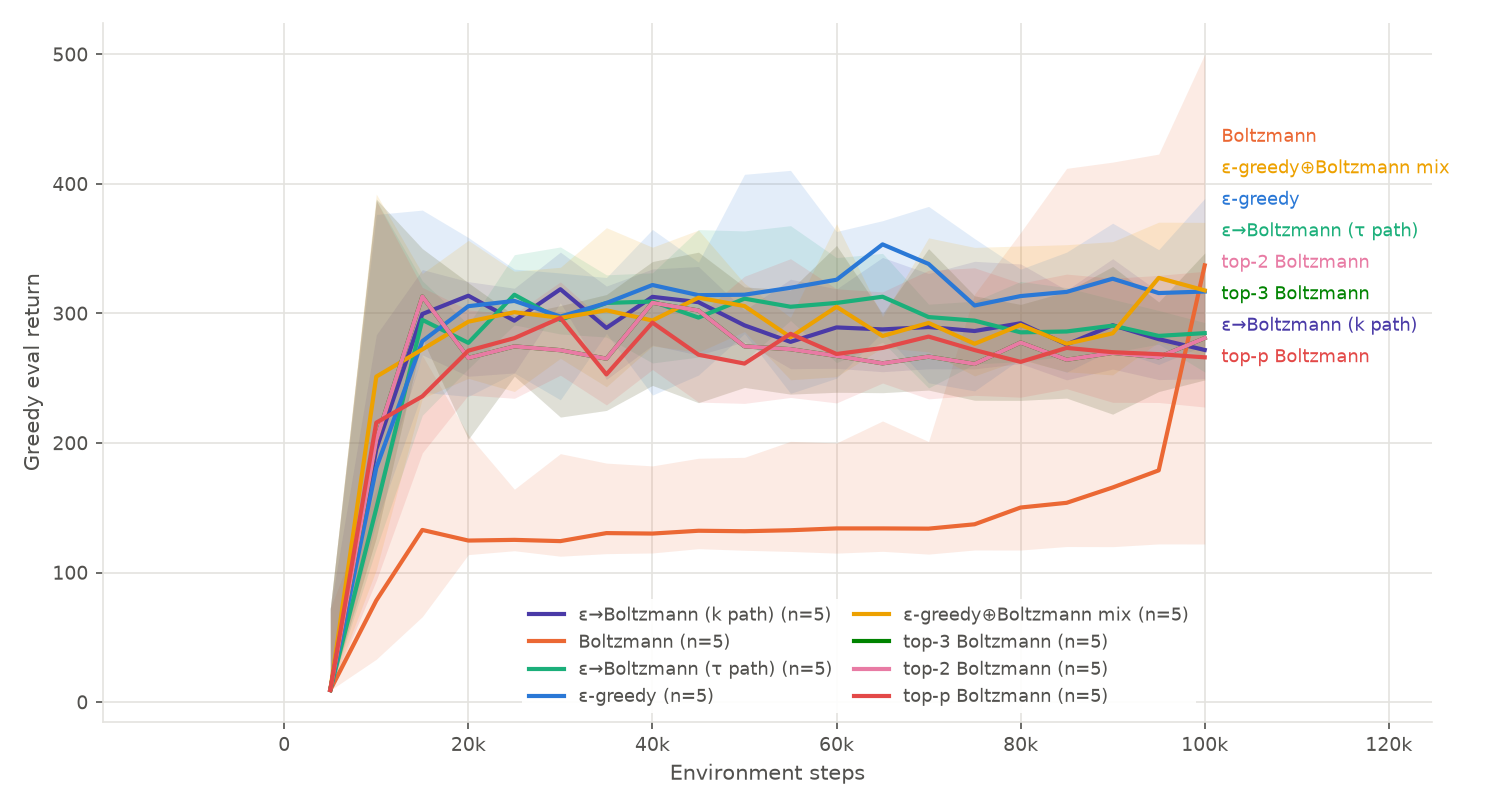
\includegraphics[width=\textwidth]{full_gym_CartPole-v1_curves.png}
  \caption{CartPole-v1}
\end{subfigure}
\hfill
\begin{subfigure}[b]{0.49\textwidth}
  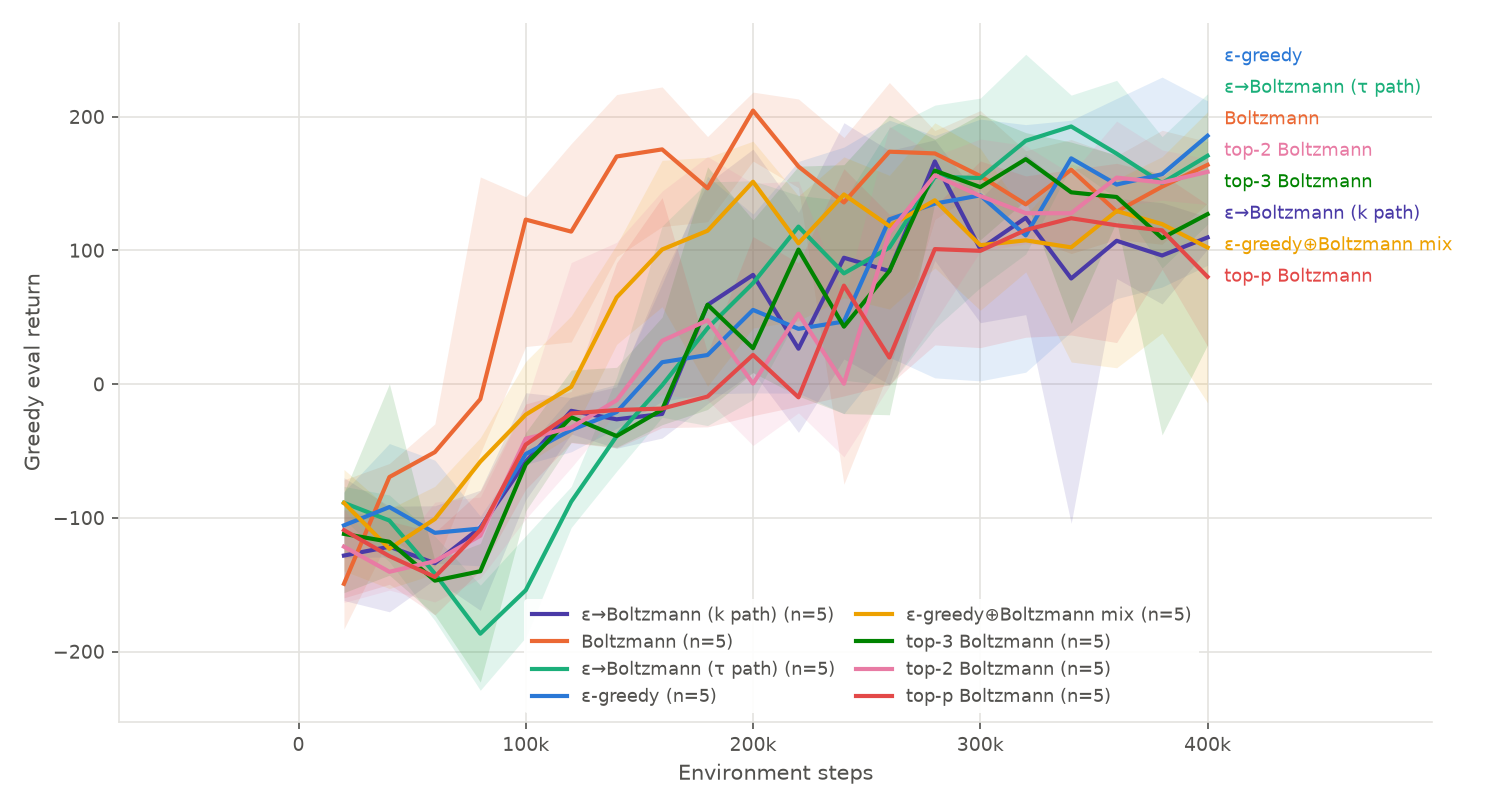
\includegraphics[width=\textwidth]{full_gym_LunarLander-v3_curves.png}
  \caption{LunarLander-v3}
\end{subfigure}
\caption{Learning curves, IQM over five seeds with bootstrap bands. The
no-floor Boltzmann variant is the slowest learner on CartPole and the fastest
on LunarLander. This sign reversal is quantified in
Table~\ref{tab:signflip}.}
\label{fig:curves}
\end{figure}

One small detail in Table~\ref{tab:main} is worth pointing out. On CartPole,
top-2 and top-3 Boltzmann are identical to the last decimal on all five seeds.
This is expected: with only two actions, both clamp to full support, so they
are the same policy. It is an unplanned end-to-end check that the top-$k$ clamp
is exact and that the pipeline is deterministic per seed.

\subsection{The $\epsilon$ floor changes sign between environments}
\label{sec:res-signflip}

Our premise was that a softmax over an untrained Q-function is worse than
uniform exploration. Measured as sample efficiency (AUC) against the
$\epsilon$-greedy baseline, the no-floor Boltzmann variant gives the numbers in
Table~\ref{tab:signflip}.

\begin{table}[h]
\centering
\small
\caption{Probability that Boltzmann without an $\epsilon$ floor beats
$\epsilon$-greedy on AUC. Both extremes exclude $0.5$ from their intervals.}
\label{tab:signflip}
\begin{tabular}{llc}
\toprule
Environment & Actions & P(Boltzmann AUC beats \eg\ AUC) \\
\midrule
CartPole-v1 & 2 & $\mathbf{0.04}$ $[0.00, 0.24]$ \quad clearly worse \\
Acrobot-v1 & 3 & $0.48$ $[0.12, 0.80]$ \quad indistinguishable \\
LunarLander-v3 & 4 & $\mathbf{0.92}$ $[0.68, 1.00]$ \quad clearly better \\
\bottomrule
\end{tabular}
\end{table}

This is the only effect in the whole main comparison that is large enough to
resolve at five seeds, and it is a sign reversal rather than a difference of
size. Dropping the $\epsilon$ floor is the worst thing you can do on CartPole
and the best thing you can do on LunarLander.

The entropy of the behaviour policy shows the mechanism (Table~\ref{tab:entropy}).

\begin{table}[h]
\centering
\small
\caption{Behaviour-policy entropy in nats, mean over five seeds. On both
environments the Boltzmann variant starts \emph{below} maximum entropy, which
is the initialisation-noise bias. What differs is what that bias costs.}
\label{tab:entropy}
\begin{tabular}{lcccc}
\toprule
& step 0 & 2k & 10k & late \\
\midrule
\multicolumn{5}{l}{\textit{CartPole, maximum entropy $\ln 2 = 0.69$; ``late'' $=$ 100k}}\\
$\epsilon$-greedy & 0.693 & 0.692 & 0.647 & 0.117 \\
Boltzmann & $\mathbf{0.569}$ & 0.559 & 0.458 & 0.163 \\
\midrule
\multicolumn{5}{l}{\textit{LunarLander, maximum entropy $\ln 4 = 1.39$; ``late'' $=$ 400k}}\\
$\epsilon$-greedy & 1.386 & 1.386 & 1.379 & 0.201 \\
Boltzmann & 1.261 & 1.261 & 1.147 & $\mathbf{0.882}$ \\
\bottomrule
\end{tabular}
\end{table}

On both environments the bias predicted in Section~\ref{sec:intro} is visible
in the very first evaluated policy. The difference is what it costs:

\begin{itemize}
\item On \textbf{CartPole} the two actions are symmetric and a random action is
      nearly free, so the early bias is pure loss and the variant never
      recovers its sample-efficiency deficit.
\item On \textbf{LunarLander} a random action is expensive. Firing thrusters at
      random crashes the lander. So the uniform floor spends the exploration
      budget on actions that are already known to be catastrophic. Boltzmann
      spends it in proportion to value instead, and still holds a useful
      $0.88$ nats of exploration at 400k steps, where $\epsilon$-greedy has
      collapsed to $0.20$.
\end{itemize}

The right way to state the premise is therefore conditional. The $\epsilon$
floor is insurance against a Q-function that is not yet informative, and like
any insurance it is worth buying only when the premium, which is the cost of a
uniformly random action, is low relative to the risk. This is a sharper claim
than ``anneal from one to the other'', and it predicts where the handover idea
should pay off: environments with many actions of widely differing cost.

\subsection{The support path wins on Acrobot}
\label{sec:res-support}

On Acrobot the support path (\texttt{anneal\_k}, $k$ grows from $1$ to $|A|$ at
fixed $\tau$) beats $\epsilon$-greedy on final return with probability of
improvement $0.96$, interval $[0.76, 1.00]$. The interval excludes $0.5$, so
this comparison is resolved. Its AUC is not better ($0.48$): it reaches a
better final policy without learning faster.

This is idea 2 from the introduction working as intended, and Acrobot is where
it should first become visible. With $|A| = 3$ it is the smallest action set
where growing the support has more than one step to take. Note that the
temperature path is at the same time the \emph{worst} variant on the same
environment ($-98.3$, $P = 0.32$), so this result is about the support path
specifically, not about annealing in general.

\subsection{What is not resolved}

Everything else. On CartPole and LunarLander every variant's probability of
improvement interval contains $0.5$, and every final-return point estimate sits
inside its neighbours' confidence intervals. $\epsilon$-greedy has the highest
point estimate on both, and that is also not a finding, because its intervals
overlap the field just as much.

\subsection{Q-scaling ablation}
\label{sec:res-ablation}

We ran the temperature-path schedule on Acrobot with the three scaling modes of
Section~\ref{sec:scale}, three seeds each. On final return, \texttt{per\_state}
gives $-151.4$ $[-237.9, -75.5]$, \texttt{running} gives $-154.5$
$[-207.1, -86.1]$, and \texttt{none} gives $-307.7$ $[-500.0, -106.9]$. The
first two are indistinguishable, and even \texttt{none} is not resolved at
three seeds.

The performance column is therefore weak. The entropy column is not, and it is
why this ablation is in the paper. Table~\ref{tab:ablation} reports the same
configurations run on two different machines.

\begin{table}[h]
\centering
\small
\caption{Q-scaling ablation on Acrobot: entropy and non-greedy action rate at
100k steps, run on two different machines. The mechanism reproduces to within
$0.04$ nats even though the performance ranking does not reproduce at all
(Section~\ref{sec:res-repro}).}
\label{tab:ablation}
\begin{tabular}{lcc}
\toprule
Mode & Entropy at 100k (4-core Linux $\to$ M1 Pro) & $P$(non-greedy) at 100k \\
\midrule
\texttt{none} & $0.93 \to \mathbf{0.90}$ & $0.46 \to \mathbf{0.45}$ \\
\texttt{running} & $0.38 \to \mathbf{0.34}$ & $0.15 \to \mathbf{0.13}$ \\
\texttt{per\_state} & $0.13 \to \mathbf{0.14}$ & $0.05 \to \mathbf{0.04}$ \\
\bottomrule
\end{tabular}
\end{table}

This is exactly what Section~\ref{sec:scale} predicts. Without normalisation
(\texttt{none}) the entropy never settles: as Q inflates from near-zero
initialisation, a fixed $\tau$ keeps meaning something different, so the policy
never converges to a stable exploration level. The one number that is supposed
to control Boltzmann exploration is not actually under the experimenter's
control. With \texttt{per\_state} the policy is about $2.5\times$ more
confidently peaked than with \texttt{running}, because forcing every Q-row to
unit spread manufactures a confident preference in rows where the actions are
genuinely equivalent.

We expected \texttt{per\_state}'s false confidence to hurt performance. On
Acrobot it does not, and we report that honestly. Reward is dense ($-1$ per
step until the goal), so early exploitation is not obviously wrong, and the
same mechanism that manufactures false confidence also cuts wasted
exploration. The mechanism is confirmed; its performance consequence is not
resolved by this data.

\subsection{The uncertainty-gated extension fails, and why}
\label{sec:res-uncertainty}

The extension of Section~\ref{sec:extension} went through three iterations. All
nine arms share seeds and architecture in one sweep. \textbf{Every gated arm
loses to the control}, and the honest headline is that the extension failed.
What follows is the diagnosis, which we think is more useful than the ranking.

The matched-architecture control does its job throughout: $\epsilon$-greedy
with the ensemble scores $-93.2$ $[-117.7, -80.3]$ against $-105.4$
$[-138.3, -81.1]$ for single-head $\epsilon$-greedy. The extra heads are, if
anything, mildly helpful, so the collapse is caused by the gating and not by
the architecture.

\paragraph{v1: the gate never fires.}
Confidence is held at $0$ during a 10k-step warm-up, then jumps and flattens.
For the ensemble signal it sits at $0.33$, $0.34$, $0.31$, $0.26$ at 12k, 20k,
50k and 100k steps, which interpolates to $\epsilon \approx 0.70$. For the TD
signal it spikes to $0.83$ and then collapses to $0.04$, giving
$\epsilon \approx 0.96$. Both arms stay between $\epsilon \approx 0.67$ and
$\epsilon \approx 0.96$ for essentially the whole run, while every fixed
schedule reaches $\epsilon \leq 0.05$ by 30k steps. The handover that the
extension exists to perform never happens, which is enough on its own to
explain the collapse. Final returns are $-385.8$ (ensemble) and $-398.5$ (TD).

\paragraph{v2: the obvious explanation, tested and falsified.}
Both signals are measured in raw Q units. Ensemble disagreement is a standard
deviation of Q-values and the TD error is a difference of them, and Q
magnitudes inflate during training. Measured over 100k steps the raw signals do
not decay, they grow: ensemble disagreement from $0.076$ to $0.136$, TD error
from $0.27$ to $1.45$. This looked like the failure mode of
Section~\ref{sec:scale} appearing somewhere Section~\ref{sec:scale} had never
been applied, so we divided the signal by the same running Q-scale the policy
uses for its temperature.

It made the signal dimensionless and changed nothing. The ratio
$u/\text{reference}$ went from $0.699 \to 0.741$ unscaled to $0.691 \to 0.831$
scaled over the same window, and final returns moved to $-375.1$ and $-312.4$,
well inside the noise. The units were a real defect but not the binding one.

\paragraph{v3: the real defect is structural.}
The ratio does not move because of how confidence was defined:
\begin{equation}
c \;=\; 1 - \frac{u}{\mathrm{quantile}(u\text{'s own recent history})}.
\label{eq:confidence}
\end{equation}
The reference is estimated \emph{from the very stream it normalises}. Whatever
$u$ does, grow or shrink or hold, the running quantile follows it, the ratio
converges to a constant, and the confidence is pinned there. This is not a
calibration error that a better learning rate would fix. No choice of units,
quantile or step size can make a self-normalising signal detect its own trend.
It was designed to be scale-free, and it came out trend-free as well.

Version 3 freezes the reference at the end of warm-up, turning it into a fixed
calibration constant measured during early training. Confidence then rises if
and only if uncertainty falls below its early-training level, which is what the
gate was always supposed to mean. Table~\ref{tab:frozen} shows the result.

\begin{table}[h]
\centering
\small
\caption{Ensemble arm with a frozen reference, mean over three seeds. The
handover finally happens: uncertainty falls, confidence rises, $\epsilon$
decays, and the Boltzmann support widens.}
\label{tab:frozen}
\begin{tabular}{lcccccc}
\toprule
& 11k & 20k & 40k & 60k & 80k & 100k \\
\midrule
uncertainty (frozen reference $= 5.25$) & 3.24 & 2.81 & 1.84 & 1.95 & 1.66 & $\mathbf{1.53}$ \\
confidence $c$ & 0.00 & 0.46 & 0.64 & 0.62 & 0.68 & $\mathbf{0.71}$ \\
$\epsilon$ & 1.00 & 0.55 & 0.37 & 0.39 & 0.33 & $\mathbf{0.30}$ \\
$k$ & 1.0 & 1.9 & 2.3 & 2.2 & 2.4 & $\mathbf{2.3}$ \\
\bottomrule
\end{tabular}
\end{table}

Final return improves from $-385.8$ to $-296.1$, and the per-seed spread is the
interesting part: one seed finishes at $-93.4$, level with the control, while
another finishes at $-500$. The mechanism can work, but it is not yet reliable.
Two problems remain, and both are now specific rather than mysterious. First,
the gate is far too slow: $\epsilon$ only reaches $0.30$ by 100k steps where
the fixed schedules reach $0.05$ by 30k, so the arm spends the whole budget
more exploratory than every competitor. Second, there is a feedback trap. A
high $\epsilon$ produces a worse value function, which produces higher
disagreement, which holds $\epsilon$ high. A measurement-driven gate closes a
loop that a time-based schedule does not.

\paragraph{The TD-error signal is unsuitable.}
With the reference frozen, the TD arm's uncertainty \emph{grows} from $8.9$ to
$24.9$ and confidence collapses to $0$. This is not a calibration problem
either. The magnitude of the TD error reflects reward scale, bootstrap noise
and target-network staleness, none of which shrink just because the agent has
learned. It is an aleatoric-flavoured signal being asked to do an epistemic
job. Ensemble disagreement, which is genuinely epistemic, falls by a factor of
two over the same window. Comparing the two signals was the point of
implementing both, and freezing the reference is what finally made the
comparison visible.

\subsection{Three seeds do not resolve a ranking}
\label{sec:res-repro}

We ran the three-seed sweeps twice on different machines: first on a four-core
Linux box, then again on the M1 Pro. Same code, same seeds, same
configurations. Only the torch and BLAS build differ, which perturbs
floating-point arithmetic enough for trajectories to diverge.

The results move a long way. On CartPole, $\epsilon$-greedy goes from $344.1$
$[303.0, 378.6]$ to $275.1$ $[218.8, 317.0]$, and no-floor Boltzmann from
$157.3$ $[108.2, 221.8]$ to $211.9$ $[113.9, 393.5]$. On Acrobot the ordering
scrambles outright: top-3 Boltzmann goes from first of eight to seventh of
eight, and the mixture variant from fifth to first.

The ordering of these variants is not stable under a change of linear algebra
library, let alone under a change of seed. Anything read out of a three-seed
ranking in this family is noise. Two things did survive the machine change
unchanged: the Q-scaling entropy mechanism of
Section~\ref{sec:res-ablation} and the gating failure of
Section~\ref{sec:res-uncertainty}. The difference between those two categories
is the line we draw in this paper between a result and a point estimate.

% ---------------------------------------------------------------------------
\section{Limitations}
\label{sec:limitations}

\begin{itemize}
\item \textbf{Five seeds resolve a sign reversal and not much else.} Only two
      comparisons in this paper have probability-of-improvement intervals that
      exclude $0.5$. Everything else is a point estimate. The deep RL
      evaluation literature asks for ten to thirty seeds
      \cite{agarwal2021,henderson2018}; we have five, and the ablation and
      extension studies have three.
\item \textbf{No Atari results.} The ALE code path is implemented and
      unit-tested but not trained; at roughly 10M frames per run, eight
      variants and five seeds is on the order of a GPU-month. This matters
      directly for our main conclusion. The mechanism in
      Section~\ref{sec:res-signflip} predicts that the effect should grow with
      the size of the action set, and Atari, with up to 18 actions, is exactly
      where that prediction should be tested.
\item \textbf{Small action sets limit idea 2.} On CartPole top-2 and top-3
      Boltzmann are provably the same policy, and \texttt{anneal\_k} has one
      step to take. Acrobot and LunarLander are better but still narrow.
\item \textbf{Three environments, all with dense rewards and low-dimensional
      observations.} They span the cost of a random action usefully, from free
      on CartPole to fatal on LunarLander, but they do not span sparse rewards,
      long horizons or pixel observations at all.
\item \textbf{One hyperparameter setting per variant.} Schedule endpoints and
      durations were chosen once by reasoning, not by search. A variant that
      looks worse may simply be badly tuned.
\item \textbf{Greedy evaluation only.} We say nothing about the online return
      an agent would actually collect while exploring, which for a deployed
      system is often the quantity that matters.
\end{itemize}

% ---------------------------------------------------------------------------
\section{Conclusion}
\label{sec:conclusion}

We asked how to hand exploration over from $\epsilon$-greedy to Boltzmann, and
we built one policy family in which both strategies are exact points, so the
handover is a well-defined path rather than an ad-hoc blend.

The clearest thing we learned is that the question is posed slightly wrongly.
It is not that Boltzmann needs to wait for a trustworthy Q-function in general.
It is that the uniform $\epsilon$ floor is insurance, and whether that
insurance is worth buying depends on how expensive a random action is in the
environment. On CartPole random actions are cheap and the floor is clearly
worth keeping; on LunarLander they crash the lander and the floor is clearly
worth dropping. Both of those comparisons are statistically resolved, and they
point in opposite directions.

Beyond that, we could resolve only one comparison among the annealing variants:
growing the softmax support beats $\epsilon$-greedy on Acrobot. We think the
most useful methodological contribution is the negative one. We show
experimentally that a three-seed ranking in this family does not survive a
change of numerical library, and we separate the claims that reproduced across
machines from the ones that did not.

Finally, the uncertainty-gated extension failed, and the reason turned out to
be a definition rather than a tuning problem: normalising a signal against a
running estimate drawn from that same signal removes the trend the gate exists
to detect. Fixing that makes the handover fire as designed, though it is still
too slow to win. We think this is worth reporting precisely because the mistake
is easy to make and invisible until you plot the reference next to the signal.

\paragraph{Reproducibility.}
All code, configurations, run outputs and figure-generating scripts are in the
accompanying repository. The main study reproduces with a single command in 35
minutes on a laptop CPU.

% ---------------------------------------------------------------------------
\begin{thebibliography}{99}

\bibitem{agarwal2021}
R.~Agarwal, M.~Schwarzer, P.~S. Castro, A.~Courville, and M.~G. Bellemare.
\newblock Deep reinforcement learning at the edge of the statistical precipice.
\newblock In \emph{Advances in Neural Information Processing Systems (NeurIPS)}, 2021.

\bibitem{bellemare2017}
M.~G. Bellemare, W.~Dabney, and R.~Munos.
\newblock A distributional perspective on reinforcement learning.
\newblock In \emph{International Conference on Machine Learning (ICML)}, 2017.

\bibitem{cesabianchi2017}
N.~Cesa-Bianchi, C.~Gentile, G.~Lugosi, and G.~Neu.
\newblock Boltzmann exploration done right.
\newblock In \emph{Advances in Neural Information Processing Systems (NIPS)}, 2017.

\bibitem{fortunato2018}
M.~Fortunato, M.~G. Azar, B.~Piot, J.~Menick, I.~Osband, A.~Graves, V.~Mnih,
  R.~Munos, D.~Hassabis, O.~Pietquin, C.~Blundell, and S.~Legg.
\newblock Noisy networks for exploration.
\newblock In \emph{International Conference on Learning Representations (ICLR)}, 2018.

\bibitem{henderson2018}
P.~Henderson, R.~Islam, P.~Bachman, J.~Pineau, D.~Precup, and D.~Meger.
\newblock Deep reinforcement learning that matters.
\newblock In \emph{AAAI Conference on Artificial Intelligence}, 2018.

\bibitem{hessel2018}
M.~Hessel, J.~Modayil, H.~van Hasselt, T.~Schaul, G.~Ostrovski, W.~Dabney,
  D.~Horgan, B.~Piot, M.~Azar, and D.~Silver.
\newblock Rainbow: Combining improvements in deep reinforcement learning.
\newblock In \emph{AAAI Conference on Artificial Intelligence}, 2018.

\bibitem{holtzman2020}
A.~Holtzman, J.~Buys, L.~Du, M.~Forbes, and Y.~Choi.
\newblock The curious case of neural text degeneration.
\newblock In \emph{International Conference on Learning Representations (ICLR)}, 2020.

\bibitem{machado2018}
M.~C. Machado, M.~G. Bellemare, E.~Talvitie, J.~Veness, M.~J. Hausknecht, and
  M.~Bowling.
\newblock Revisiting the Arcade Learning Environment: Evaluation protocols and
  open problems for general agents.
\newblock \emph{Journal of Artificial Intelligence Research}, 61:523--562, 2018.

\bibitem{mnih2015}
V.~Mnih, K.~Kavukcuoglu, D.~Silver, A.~A. Rusu, J.~Veness, M.~G. Bellemare,
  A.~Graves, M.~Riedmiller, A.~K. Fidjeland, G.~Ostrovski, et~al.
\newblock Human-level control through deep reinforcement learning.
\newblock \emph{Nature}, 518(7540):529--533, 2015.

\bibitem{osband2016}
I.~Osband, C.~Blundell, A.~Pritzel, and B.~Van~Roy.
\newblock Deep exploration via bootstrapped DQN.
\newblock In \emph{Advances in Neural Information Processing Systems (NIPS)}, 2016.

\bibitem{schaul2016}
T.~Schaul, J.~Quan, I.~Antonoglou, and D.~Silver.
\newblock Prioritized experience replay.
\newblock In \emph{International Conference on Learning Representations (ICLR)}, 2016.

\bibitem{sutton2018}
R.~S. Sutton and A.~G. Barto.
\newblock \emph{Reinforcement Learning: An Introduction}.
\newblock MIT Press, 2nd edition, 2018.

\bibitem{towers2024}
M.~Towers, A.~Kwiatkowski, J.~Terry, J.~U. Balis, G.~De~Cola, T.~Deleu,
  M.~Goul\~{a}o, A.~Kallinteris, M.~Krimmel, A.~KG, et~al.
\newblock Gymnasium: A standard interface for reinforcement learning
  environments.
\newblock \emph{arXiv preprint arXiv:2407.17032}, 2024.

\bibitem{vanhasselt2016}
H.~van Hasselt, A.~Guez, and D.~Silver.
\newblock Deep reinforcement learning with double Q-learning.
\newblock In \emph{AAAI Conference on Artificial Intelligence}, 2016.

\bibitem{wang2016}
Z.~Wang, T.~Schaul, M.~Hessel, H.~van Hasselt, M.~Lanctot, and N.~de~Freitas.
\newblock Dueling network architectures for deep reinforcement learning.
\newblock In \emph{International Conference on Machine Learning (ICML)}, 2016.

\end{thebibliography}

\end{document}
